% ---
% tags: [AI Infra, 集群, KV Cache]
% author: marshall
% excerpt:
% ---
\documentclass[11pt]{article}

\usepackage{fontspec}
\usepackage{xeCJK}
% macOS 上 SimSun 位于 Microsoft Word 内部；如需其它字体请修改下面路径
\setCJKmainfont[Path=/Applications/Microsoft Word.app/Contents/Resources/DFonts/, Extension=.ttc]{Simsun}

\usepackage[a4paper, margin=2.2cm]{geometry}
\linespread{1.3}
\setlength{\parskip}{0.3em}
\usepackage{amsmath, amssymb, amsthm}
\usepackage{graphicx}
% 本文图片统一放在与 .tex 同名的文件夹 latex/<slug>/ 中，直接用文件名引用即可
\graphicspath{{./}{2026-11-23-deepinfer-beyond/}}
\usepackage{hyperref}
\hypersetup{colorlinks=true, linkcolor=blue, urlcolor=blue}

\title{DeepInfer之外：房间里的大象——集群Infra}
\author{Marshall}

\begin{document}
\maketitle

DeepInfer 开源之后，社区把很多注意力放在了它释放出来的引擎层能力上：FlashMLA、DeepGEMM、DeepEP、DSpark 投机解码，以及 SWA Bounded Replay 等等。但如果你仔细看 DeepInfer 仓库的 README，就会发现它在最后列了三件“本次开源未包含、但完整在线服务必须具备”的东西：\textbf{KV Cache 系统}、\textbf{VE/Prefill/Decode 分离部署}，以及 \textbf{跨 DP 副本的负载均衡}。

而它没有开源的那一半，恰恰就是支撑千卡规模线上服务的“房间里的大象”——\textbf{集群 Infra}。

\section{集群会带来什么新问题？}

如果我们把视角从单实例拉到千卡集群，会发现单机优化和集群现实之间有四个很典型的错配：

\begin{enumerate}
  \item \textbf{负载均衡的局部最优陷阱}：单实例的 Continuous Batching 只看自己卡上的队列，但集群里有几十上百个实例。如果 Gateway 还是按轮询（Round-Robin）或连接数分发，长短请求混在一起，一个 128K 的 Prefill 就能把整组实例的 TPOT 拖垮；更糟的是，Prefix Cache 命中率会因为路由随机而直接腰斩。

  \item \textbf{PD / AF 分离后的“网络与存储债”}：单机引擎把 Prefill 和 Decode 拆开，把计算和访存最优化了，但代价是\textbf{把原本在卡内 HBM 解决的 KV Cache，变成了跨节点的实时网络传输}。如果集群网络（RoCE/IB）和传输引擎跟不上，TTFT 里省下来的算力全会赔在 KV 搬运的排队和尾延迟上。

  \item \textbf{潮汐流量下的算力闲置}：线上推理流量天然有昼夜潮汐（白天高并发，凌晨低谷），如果集群按峰值静态划死给推理，夜间大量 H800/B200 只能空转；如果和训练/离线任务混部，又面临秒级/分钟级的冷启动与权重加载延迟。

  \item \textbf{大 EP 与超节点下的故障半径放大}：以前单机 8 卡挂一张卡，最多影响一个实例；现在 Decode 拉到 EP144（18 台 8 卡机绑成一个部署单元），只要其中任意一台机器的网卡抖动或显存 ECC 报错，整个 144 卡的同步点全得卡死或重拉。
\end{enumerate}

\section{全局路由与分布式 KV 池：从“无状态转发”到“以 KV 为中心”}

传统微服务网关的假设是“请求无状态，哪个后端闲就发给谁”。但在长上下文、Agent 多轮对话和 System Prompt 复用的场景下，\textbf{KV Cache 本身就是最贵的状态}——重算一遍 100K 上下文的 Prefill 要几秒钟和大量 FLOPs，而从远端 DRAM/SSD 甚至邻近节点的 HBM 拉过来只需要几十毫秒。

于是集群调度正在从“以计算为中心”转向 \textbf{“以 KVCache 为中心（KVCache-centric）”}，典型代表就是 Mooncake 和 NVIDIA Dynamo 的架构思路：

\begin{figure}[htbp]
  \centering
  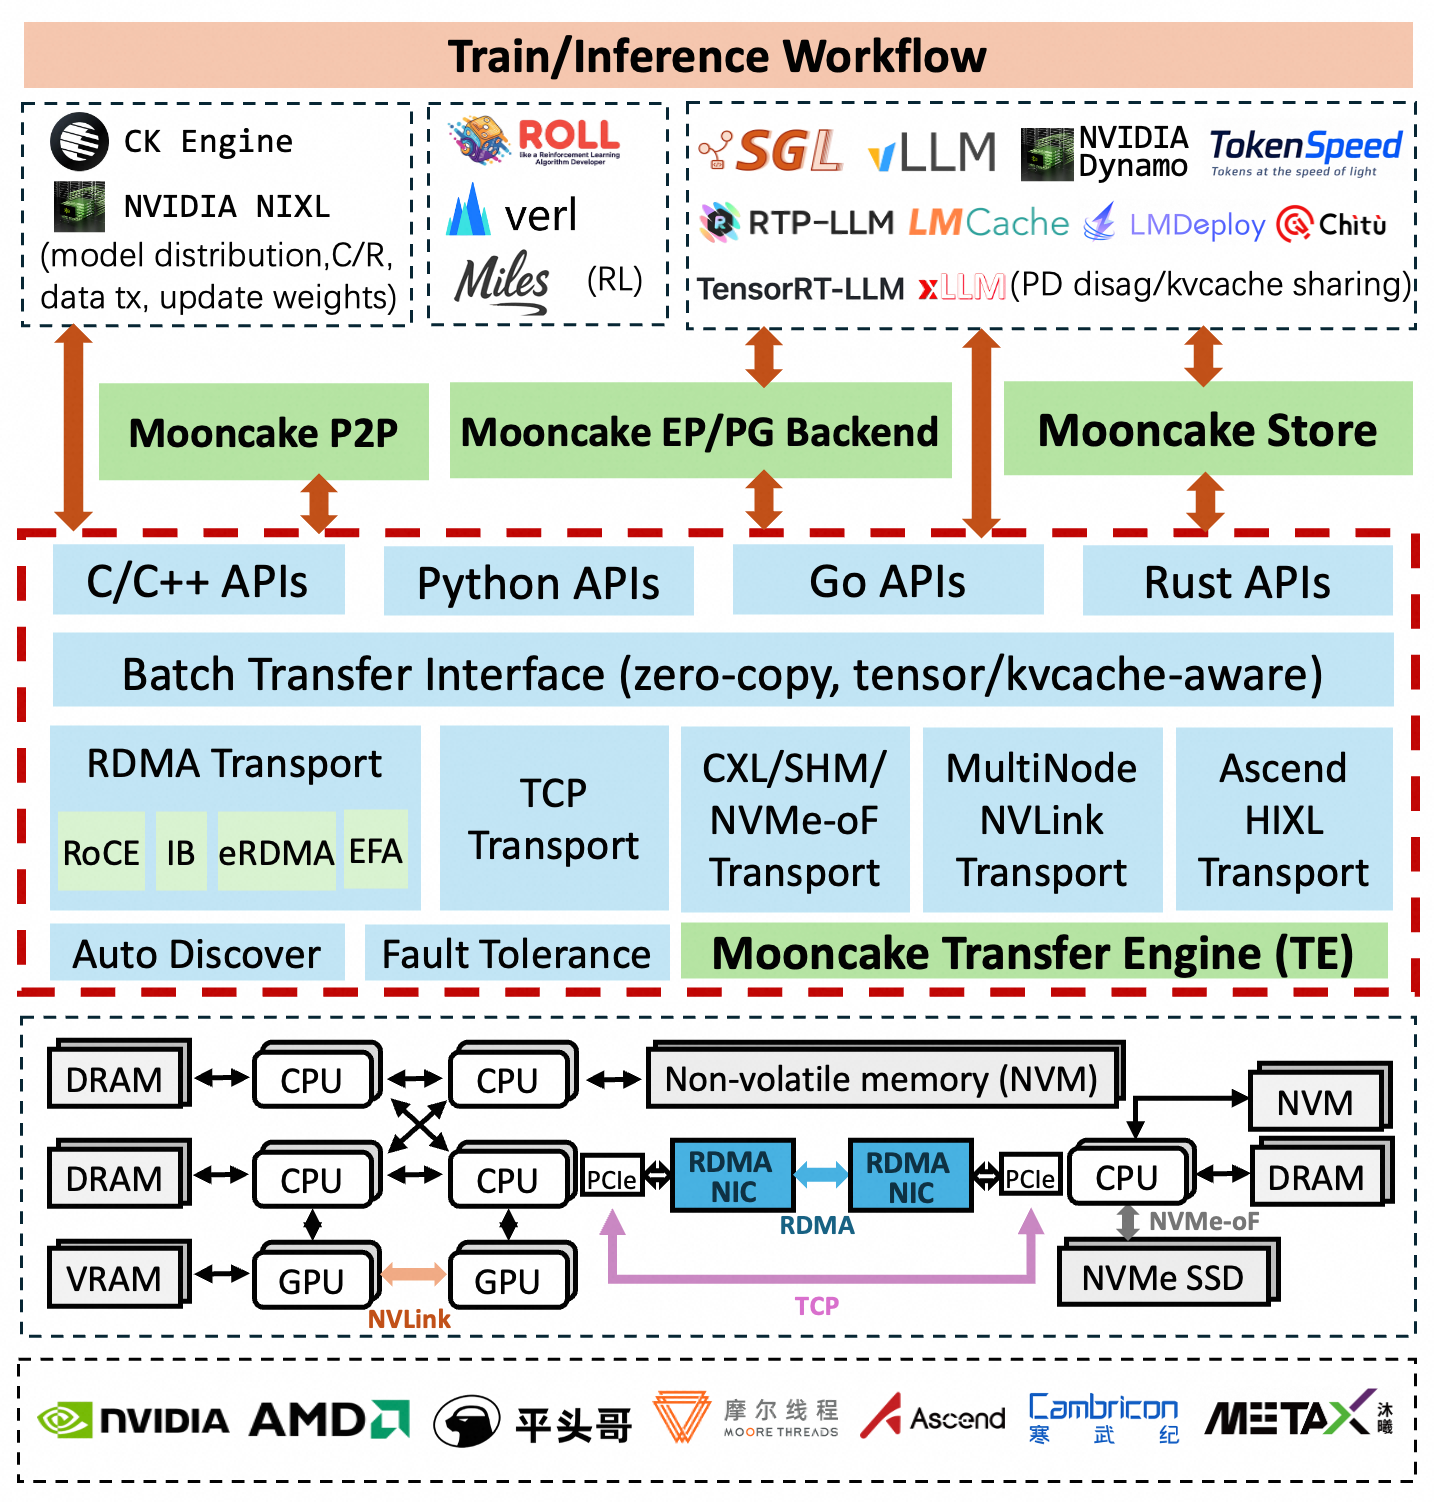
\includegraphics[width=0.85\textwidth]{mooncake-components.png}
  \caption{Mooncake 组件架构}
  \label{fig:mooncake-components}
\end{figure}

\begin{enumerate}
  \item \textbf{KV-Aware Router（缓存感知路由）}：

  Gateway 不再盲目轮询，而是维护一张全局（或近似实时）的 Prefix Cache 分布表。新请求进来时，先算前缀哈希，优先路由到已经缓存了对应 Prefix 的节点上；同时结合该节点当前的排队长度和显存水位做打分，在“缓存命中收益”和“计算排队代价”之间做权衡。

  \item \textbf{多级分布式 KV 池（HBM → DRAM → SSD / 3FS）}：

  单卡 HBM 永远不够放所有活跃用户的历史对话。集群 Infra 把各台机器闲置的主机内存（DRAM）和本地 NVMe SSD（或像 DeepSeek 3FS 这样的并行文件系统）池化起来，构成 L2/L3 KV Cache。以 DeepSeek-V3/R1 线上统计为例，24 小时内 608B 输入 token 中有 \textbf{342B（56.3\%）命中了磁盘上的 KV Cache}，直接省掉了超过一半的 Prefill 算力。

  \item \textbf{跨节点零拷贝传输引擎（Mooncake Transfer Engine / NIXL）}：

  有了分布式 KV 池和 PD 分离，数据搬运就成了热路径。无论是 Mooncake 的 Transfer Engine 还是 Dynamo 的 NIXL，核心都是在做同一件事：\textbf{绕过 CPU 内存拷贝，直接用 RDMA / GPUDirect Storage / NVLink 把 KV Block 从 Prefill 卡的 HBM 或远端 DRAM/SSD 直接写进 Decode 卡的 HBM}。
\end{enumerate}

\begin{figure}[htbp]
  \centering
  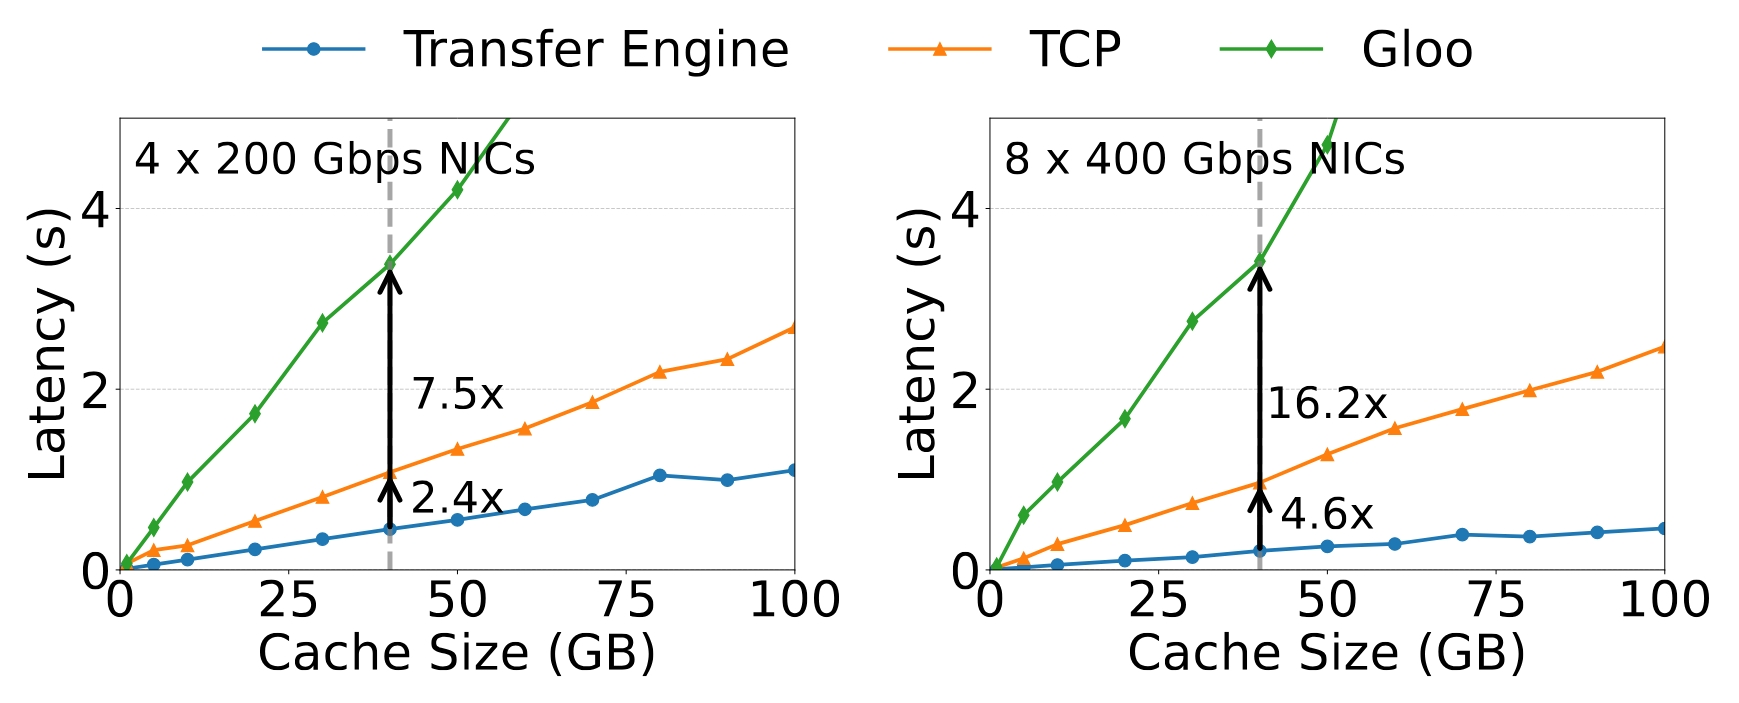
\includegraphics[width=0.85\textwidth]{mooncake-transfer.png}
  \caption{Mooncake 传输性能}
  \label{fig:mooncake-transfer}
\end{figure}

\section{集群资源编排：潮汐混部、SLA 驱动扩缩容与快速冷启动}

有了路由和 KV 传输，下一个现实问题是：\textbf{集群里到底该放多少台 Prefill、多少台 Decode，以及白天晚上怎么变？}

\begin{table}[htbp]
  \centering
  \small
  \begin{tabular}{p{2.4cm}p{3.4cm}p{5.0cm}p{4.1cm}}
    \hline
    \textbf{集群编排能力} & \textbf{传统静态集群做法} & \textbf{现代推理集群 Infra 做法} & \textbf{解决的核心痛点} \\
    \hline
    PD 配比与扩缩容 & 人工按经验配固定比例（如 1:3） & SLA 驱动的 Planner（如 Dynamo Planner）按 TTFT/ITL 实时调配 P/D 池大小 & 避免输入/输出长度分布变化导致一侧排队、另一侧空转 \\
    \hline
    昼夜潮汐调度 & 按峰值常驻，夜间低利用率空转 & 白天全量接推理，夜间自动缩容把节点让渡给离线训练/研究 & 拉平 24 小时集群 TCO，把夜间闲置算力变现 \\
    \hline
    副本冷启动 & 从对象存储/NAS 拉几十 GB 权重到 CPU 再进 GPU（分钟级） & GPU-to-GPU 权重流式广播（如 ModelExpress / RDMA 直传，秒级） & 支撑突发流量下的快速扩容与故障实例秒级拉起 \\
    \hline
    拓扑感知调度 & K8s 默认调度，随机打散 Pod & 拓扑感知 Gang Scheduling（如 Grove，对齐 NVL72 / IB 交换机域） & 防止 EP144/NVL72 被打散到跨机架，避免跨核心交换机拥塞 \\
    \hline
  \end{tabular}
\end{table}

拿 DeepSeek 公布的 24 小时线上节点数变化来看，这种“潮汐混部”在真实生产环境里已经非常成熟：白天高峰期 V3/R1 推理服务占满 \textbf{278 个 8×H800 节点}，到夜间低谷期逐步缩容，把空出来的节点直接切回研究和训练任务，24 小时平均占用控制在 \textbf{226.75 个节点}。

\begin{figure}[htbp]
  \centering
  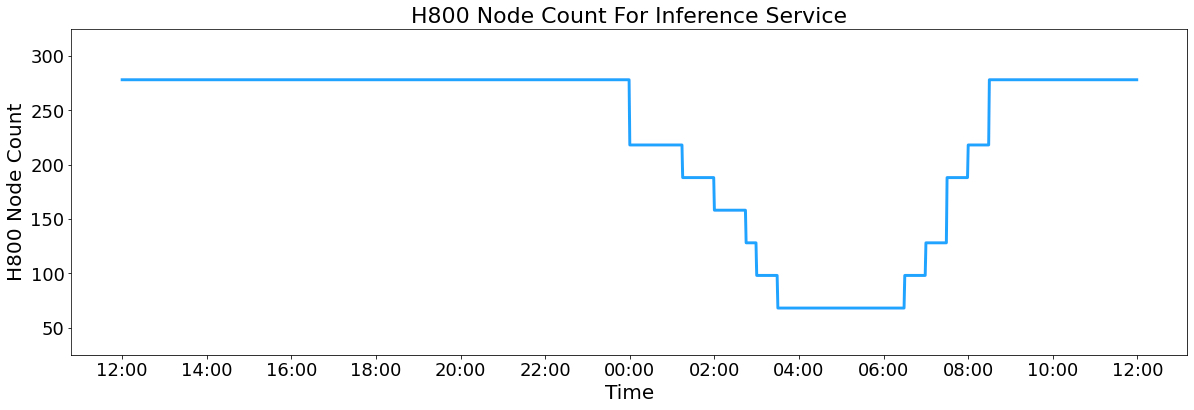
\includegraphics[width=0.85\textwidth]{h800-tide.jpg}
  \caption{H800 节点昼夜潮汐变化}
  \label{fig:h800-tide}
\end{figure}

\section{高可用与故障域控制}

在大 EP（比如 EP144）和 PD 分离架构下，系统的脆弱性比以前高得多：

\begin{itemize}
  \item \textbf{以前}：一个 8 卡 TP 实例挂了，K8s 重启这 1 台机器，影响面是单个实例的几个并发请求。
  \item \textbf{现在}：一个 Decode 部署单元横跨 18 台机器（144 张卡），它们在每一层都要做 All-to-All 同步。只要其中 1 张卡掉卡、或者 1 根光模块闪断，整个 144 卡实例都会卡在 \texttt{Dispatch/Combine} 的屏障上。
\end{itemize}

因此，集群 Infra 必须补齐三道防线：

\begin{enumerate}
  \item \textbf{In-flight 请求迁移（Request Migration）}：

  当某个 Decode 节点出现健康检查异常或硬件降级时，控制面不能直接把正在生成的长请求掐断报错，而是要能把该请求已经生成的 token 和对应的 KV 状态（通过分布式 KV 池或对等节点）无缝迁移到健康的 Decode 实例上继续吐字。

  \item \textbf{局部隔离与无感摘除}：

  Router 和控制面需要亚秒级的金丝雀探针与慢节点识别（Slow-rank detection），一旦发现某台机器的 RDMA 重传率飙升或算力降频，立刻将其从路由表摘除并触发替换，防止一个慢节点把整条流水线拖成慢吞吞的同步队尾。

  \item \textbf{跨集群容灾与多租户隔离}：

  在 RDMA 网络上，训练流量（大包、高带宽、突发性强）和推理流量（小包、低延迟敏感）如果混跑在同一张网卡或同一个 Virtual Lane 上，训练的 AllReduce 瞬间就能把推理的 DeepEP 延迟打爆。生产集群通常需要通过 \textbf{InfiniBand VL（Virtual Lane）或 RoCE DSCP/PFC 队列隔离}，把推理控制面、KV 传输和训练流量彻底隔开。
\end{enumerate}

\section{小结}

今天头部推理系统的演进已经很清楚：单机引擎负责把算子和微批流水线压到极致，而引擎之上的 \textbf{KV 感知路由、分布式多级 KV 池、RDMA 零拷贝传输、潮汐混部编排以及大 EP 故障迁移}，正在把原本分散的 GPU 节点真正转变成一台“数据中心级推理计算机”。

\end{document}
